\documentclass{article}
\usepackage[T1]{fontenc}
\usepackage[utf8]{inputenc}
\usepackage[polish]{babel}
\usepackage{amsmath}
\usepackage{url}
\usepackage{graphicx}
 \usepackage{float}
 \usepackage{pgfplots}
\pgfplotsset{compat=1.18}
%{Informatyka stosowana 2022, I st., semestr VI}


\author{
	{Dominik Gałkowski, 247659} \\
	{Jan Śladowski, 247806}\\ 
{Prowadzący: dr inż. Marcin Kacprowicz}
}

\title{Komputerowe systemy rozpoznawania 2024/2025\\Projekt 2. Podsumowania lingwistyczne relacyjnych baz danych}
\begin{document}
\maketitle 

\section{Cel}
Celem projektu jest stworzenie aplikacji, której główną funkcjonalnością
jest lingwistyczna agregacja zawartości wybranego zbioru danych. Ma ona za zadanie generowanie podsumowań lingwistycznych dla wybranych przez użytkownika kwantyfikatorów, sumaryzatorów i kwalifikatorów dla różnych atrybutów. Analiza otrzymanych wyników polega na określeniu, znaczenia wybranych kwantyfikatorów, sumaryzatorów, kwalifikatorów oraz miar ich jakości dla wiarygodności i jakości otrzymanych podsumowań lingwistycznych. Przykładowe podsumowanie to, np. większość pomiarów ma wysokie ciśnienie.


\section{Baza danych, zmienne lingwistyczne, kwantyfikatory lingwistyczne}

\subsection{Charakterystyka podsumowywanej bazy danych}
W tym projekcie został wykorzystany zbiór danych zapisany w pliku w formacie .csv, na podstawie którego utworzono bazę danych - PostgresSQL. Baza danych o nazwie World Weather Repository zawiera różnego rodzaju pomiary danych atmosferycznych, np. temperatura lub prędkość wiatru. \cite{baza} Użteczność bazy jest określona na stronie Kaggle jako 10.0, a dane z niej są wykorzystywane do prognozowanie pogody oraz analizy klimatu na różnych kontynentach. Baza jest nabieżąco aktualizowana, natomiast na dzień 18.05.2025r. składa się z 62603 rekordów. 

Zmiennym lingwistycznym przypisuje się znaczenie ze względu na potrzebę lepszej interpretowalności danych przez użytkowników. Ludzie rzadko reagują na dokładne wartości (np. 1033.8 mb ciśnienia), natomiast określenie „wysokie ciśnienie” pozwala im intuicyjnie rozumieć sytuację pogodową. Stąd istnieje zapotrzebowanie na „przekładanie” danych formalnych na język naturalny. \\
Podmiotem podsumowań jest pomiar atmosferyczny, z bazy World Weather Repository wybrano 10 atrybutów, które zostaną rozmyte, są to następujące kolumny: last\_updated, temperature\_celsius, wind\_kph, pressure\_mb, humidity, visibility\_km, uv\_index, air\_quality\_Carbon\_Monoxide,  \\air\_quality\_Nitrogen\_dioxide, air\_quality\_gb\_defra\_index \\
Dokładne opisy atrybutów znajdują się w załączniku pod nazwą załącznik1.pdf.

\subsection{Zmienne lingwistyczne (atrybuty/własności obiektów)}
Poniżej zostały zaprezentowane zmienne lingwistyczne dla atrybutów opisanych w sekcji 2.1 oraz ich wzory analityczne. W każdym z poniższych wzorów \(L_x\) to zmienna ligwistyczna, $\mathcal{L}_x$ - nazwa zmiennej lingwistycznej , \(H_x\) zbiór możliwych przyjmowanych wartości, \(X_x\) - przestrzeń rozważań, \(x\) - numer kolejnej zmiennej lingwistycznej. 
\begin{enumerate}
    \item last\_updated
        \begin{equation}
            L_1 = \langle \mathcal{L}_1, H_1, \mathcal{X}_1 \rangle
        \end{equation}
        gdzie: $\mathcal{L}_1$ – pora dnia, $H_1$ – \{nocna, poranna, południowa, popołudniowa, wieczorna\}, $\mathcal{X}_1 = [0, 24]$. \\
        Poniżej wzory dla wszystkich możliwych etykiet.
        \begin{equation}
            \mu_{\text{nocna}}(x) =
            \begin{cases}
            \frac{7 - x}{3}, & x \in (4, 7) \\
            1, & x \in [0, 4] \\
            \frac{x - 21}{3}, & x \in [21, 24) \\
            0, & \text{w przeciwnym razie} \\
            \end{cases}
        \end{equation}

        \begin{equation}
            \mu_{\text{poranna}}(x) =
            \begin{cases}
            \frac{x - 4}{3}, & x \in (4, 7) \\
            1, & x \in [7, 9] \\
            \frac{12 - x}{3}, & x \in (9, 12) \\
            0, & \text{w przeciwnym razie} \\
            \end{cases}
        \end{equation}

        \begin{equation}
            \mu_{\text{południowa}}(x) =
            \begin{cases}
            \frac{x - 9}{3}, & x \in (9, 12) \\
            1, & x \in [12, 13] \\
            \frac{16 - x}{3}, & x \in (13, 16) \\
            0, & \text{w przeciwnym razie} \\
            \end{cases}
        \end{equation}

        \begin{equation}
            \mu_{\text{popołudniowa}}(x) =
            \begin{cases}
            \frac{x - 13}{3}, & x \in (13, 16) \\
            1, & x \in [16, 17] \\
            \frac{20 - x}{3}, & x \in (17, 20) \\
            0, & \text{w przeciwnym razie} \\
             \end{cases}
        \end{equation}

        \begin{equation}
            \mu_{\text{wieczorna}}(x) =
            \begin{cases}
            \frac{x - 17}{3}, & x \in (17, 20) \\
            1, & x \in [20, 21] \\
            \frac{24 - x}{3}, & x \in (21, 24) \\
            0, & \text{w przeciwnym razie} \\
            \end{cases}
        \end{equation} 
        
Wykres funkcji przynależności znajduje się w załączniku pod nazwą img/day.png.
    
    \item temperature\_celsius
        \begin{equation}
            L_2 = \langle \mathcal{L}_2, H_2, \mathcal{X}_2 \rangle
        \end{equation}
        gdzie: $\mathcal{L}_2$ – temperatura, $H_2$ – \{bardzo zimna, zimna, umiarkowana, ciepła, gorąca\}, $\mathcal{X}_2 = [-25, 50]$. \\
        Poniżej wzory dla wszystkich możliwych etykiet.
                \begin{equation}
                   \mu_{\text{bardzo\_zimna}}(x) =
                    \begin{cases}
                    1, & x \in [-25, -15] \\
                    \frac{-5 - x}{10}, & x \in (-15, -5) \\
                    0, & \text{w przeciwnym razie}
                    \end{cases}
                \end{equation}
                
                \begin{equation}
                   \mu_{\text{zimna}}(x) =
                    \begin{cases}
                    \frac{x + 10}{10}, & x \in (-15, -5) \\
                    1, & x \in [-5, 0] \\
                    \frac{10 - x}{10}, & x \in (0, 10) \\
                    0, & \text{w przeciwnym razie}
                    \end{cases}
                \end{equation}

                \begin{equation}
                    \mu_{\text{umiarkowana}}(x) =
                    \begin{cases}
                    \frac{x}{10}, & x \in (0, 10) \\
                    1, & x \in [10, 15] \\
                    \frac{20 - x}{10}, & x \in (15, 25) \\
                    0, & \text{w przeciwnym razie}
                    \end{cases}
                \end{equation}

                \begin{equation}
                    \mu_{\text{ciepła}}(x) =
                    \begin{cases}
                    \frac{x - 15}{10}, & x \in (15, 25) \\
                    1, & x \in [25, 30] \\
                    \frac{30 - x}{10}, & x \in (30, 40) \\
                    0, & \text{w przeciwnym razie}
                    \end{cases}
                \end{equation}

                \begin{equation}
                    \mu_{\text{gorąca}}(x) =
                    \begin{cases}
                    \frac{x - 30}{10}, & x \in (30, 40] \\
                    1, & x \in 40, 50] \\
                    0, & \text{w przeciwnym razie}
                    \end{cases}
                \end{equation}

Wykres funkcji przynależności znajduje się w załączniku pod nazwą img/temp.png.

    \item wind\_kph
        \begin{equation}
            L_3 = \langle \mathcal{L}_3, H_3, \mathcal{X}_3 \rangle
        \end{equation}
        gdzie: $\mathcal{L}_3$ – wiatr, $H_3$ – \{słaby, umiarkowany, silny, bardzo silny, gwałtowny\}, $\mathcal{X}_3 = [3, 151]$. \\
        Poniżej wzory dla wszystkich możliwych etykiet.
                  \begin{equation}
                    \mu_{\text{słaby}}(x) =
                    \begin{cases}
                    1, & x = 0 \\
                    \frac{20 - x}{20}, & x \in (0, 20) \\
                    0, & \text{w przeciwnym razie}
                    \end{cases}
                  \end{equation}
                \begin{equation}
                    \mu_{\text{umiarkowany}}(x) =
                    \begin{cases}
                    \frac{x}{20}, & x \in (0, 20) \\
                    1, & x = 20 \\
                    \frac{40 - x}{20}, & x \in (20, 40) \\
                    0, & \text{w przeciwnym razie}
                    \end{cases}
                  \end{equation}
                \begin{equation}
                    \mu_{\text{silny}}(x) =
                    \begin{cases}
                    \frac{x - 20}{20}, & x \in (20, 40) \\
                    1, & x = 40 \\
                    \frac{60 - x}{20}, & x \in (40, 60) \\
                    0, & \text{w przeciwnym razie}
                    \end{cases}
              \end{equation}
                \begin{equation}
                    \mu_{\text{bardzo\_silny}}(x) =
                    \begin{cases}
                    \frac{x - 40}{20}, & x \in (40, 60) \\
                    1, & x = 60 \\
                    \frac{75 - x}{15}, & x \in (60, 75) \\
                    0, & \text{w przeciwnym razie}
                    \end{cases}
              \end{equation}
              \begin{equation}
                    \mu_{\text{gwałtowny}}(x) =
                    \begin{cases}
                    \frac{x - 60}{15}, & x \in (60, 75) \\
                    1, & x \in [75, 81] \\
                    0, & \text{w przeciwnym razie}
                    \end{cases}
              \end{equation}

Wykres funkcji przynależności znajduje się w załączniku pod nazwą img/wind.png.
              
    \item pressure\_mb
        \begin{equation}
            L_4 = \langle \mathcal{L}_4, H_4, \mathcal{X}_4 \rangle
        \end{equation}
        gdzie: $\mathcal{L}_4$ – ciśnienie, $H_4$ – \{niskie, normalne, wysokie\}, $\mathcal{X}_4 = [947, 1050]$. \\
        Poniżej wzory dla wszystkich możliwych etykiet.
                \begin{equation}
                    \mu_{\text{niskie}}(x) =
                    \begin{cases}
                    1, & x \in [964, 970] \\
                    \frac{1000 - x}{30}, & x \in (970, 1000] \\
                    0, & \text{w przeciwnym razie}
                    \end{cases}
              \end{equation}
                \begin{equation}
                   \mu_{\text{normalne}}(x) =
                    \begin{cases}
                    \frac{x - 970}{30}, & x \in (970, 1000] \\
                    1, & x \in (1000, 1020] \\
                    \frac{1040 - x}{20}, & x \in (1020, 1040] \\
                    0, & \text{w przeciwnym razie}
                    \end{cases}
                \end{equation}

                \begin{equation}
                \mu_{\text{wysokie}}(x) =
                    \begin{cases}
                    \frac{x - 1020}{20}, & x \in (1020, 1040] \\
                    1, & x \in (1040, 1052] \\
                    0, & \text{w przeciwnym razie}
                    \end{cases}
                \end{equation}

Wykres funkcji przynależności znajduje się w załączniku pod nazwą img/pressure.png.
    
    \item humidity
    \begin{equation}
            L_5 = \langle \mathcal{L}_5, H_5, \mathcal{X}_5 \rangle
        \end{equation}
        gdzie: $\mathcal{L}_5$ – wilgotność powietrza, $H_5$ – \{suche, umiarkowane, wilgotne\}, $\mathcal{X}_1 = [2, 100]$. \\
        Poniżej wzory dla wszystkich możliwych etykiet.

        \begin{equation}
        \mu_{\text{sucho}}(x) =
        \begin{cases}
        1, & x \in (0, 10] \\
        \frac{50 - x}{40}, & x \in (10, 50) \\
        0, & \text{w przeciwnym razie}
        \end{cases}
        \end{equation}

        \begin{equation}
        \mu_{\text{umiarkowane}}(x) =
        \begin{cases}
        \frac{x - 10}{40}, & x \in (10, 50) \\
        1, & x = 50 \\
        \frac{80 - x}{30}, & x \in (50, 80) \\
        0, & \text{w przeciwnym razie}
        \end{cases}
        \end{equation}

        \begin{equation}
        \mu_{\text{wilgotne}}(x) =
        \begin{cases}
        \frac{x - 50}{30}, & x \in (50, 80) \\
        1, & x \in [80, 100] \\
        0, & \text{w przeciwnym razie}
        \end{cases}
        \end{equation}

Wykres funkcji przynależności znajduje się w załączniku pod nazwą img/humidity.png.

    \item visibility\_km
    \begin{equation}
            L_6 = \langle \mathcal{L}_6, H_6, \mathcal{X}_6 \rangle
        \end{equation}
        gdzie: $\mathcal{L}_6$ – stopień widoczności, $H_6$ – \{słaba, umiarkowana, dobra, bardzo dobra\}, $\mathcal{X}_6 = [0, 32]$. \\
        Poniżej wzory dla wszystkich możliwych etykiet.
        
    \begin{equation}
    \mu_{\text{słaba}}(x) =
    \begin{cases}
    1, & x \in [0, 2] \\
    \frac{6 - x}{4}, & x \in (2, 6] \\
    0, & \text{w przeciwnym razie}
    \end{cases}
    \end{equation}
    
    \begin{equation}
    \mu_{\text{umiarkowana}}(x) =
    \begin{cases}
    \frac{x - 2}{4}, & x \in (2, 6] \\
    1, & x \in (6, 10] \\
    \frac{14 - x}{4}, & x \in (10, 14] \\
    0, & \text{w przeciwnym razie}
    \end{cases}
    \end{equation}
    
    \begin{equation}
    \mu_{\text{dobra}}(x) =
    \begin{cases}
    \frac{x - 10}{4}, & x \in (10, 14) \\
    1, & x \in [14, 18] \\
    \frac{22 - x}{4}, & x \in (18, 22) \\
    0, & \text{w przeciwnym razie}
    \end{cases}
    \end{equation}

    \begin{equation}
    \mu_{\text{bardzo\_dobra}}(x) =
    \begin{cases}
    \frac{x - 18}{4}, & x \in (18, 22) \\
    1, & x \in [22, 24] \\
    0, & \text{w przeciwnym razie}
    \end{cases}
    \end{equation}

Wykres funkcji przynależności znajduje się w załączniku pod nazwą img/visibility.png.

    \item uv\_index
    \begin{equation}
            L_7 = \langle \mathcal{L}_7, H_7, \mathcal{X}_7 \rangle
        \end{equation}
        gdzie: $\mathcal{L}_7$ – promieniowanie UV, $H_1$ – \{niskie, umiarkowane, wysokie, bardzo wysokie, ekstremalne\}, $\mathcal{X}_7 = [0, 16]$. \\
        Poniżej wzory dla wszystkich możliwych etykiet.

    \begin{equation}
    \mu_{\text{niskie}}(x) =
    \begin{cases}
    1, & x \in [0, 2] \\
    \frac{3 - x}{1}, & x \in (2, 3] \\
    0, & \text{w przeciwnym razie}
    \end{cases}
    \end{equation}
    
    \begin{equation}
    \mu_{\text{umiarkowane}}(x) =
    \begin{cases}
    \frac{x - 2}{1}, & x \in (2, 3] \\
    1, & x \in (3, 5] \\
    \frac{6 - x}{1}, & x \in (5, 6) \\
    0, & \text{w przeciwnym razie}
    \end{cases}
    \end{equation}
    
    \begin{equation}
    \mu_{\text{wysokie}}(x) =
    \begin{cases}
    \frac{x - 5}{1}, & x \in (5, 6] \\
    1, & x \in (6, 7] \\
    \frac{8 - x}{1}, & x \in (7, 8) \\
    0, & \text{w przeciwnym razie}
    \end{cases}
    \end{equation}
    
    \begin{equation}
    \mu_{\text{bardzo\_wysokie}}(x) =
    \begin{cases}
    \frac{x - 7}{1}, & x \in (7, 8] \\
    1, & x \in (8, 10] \\
    \frac{11 - x}{1}, & x \in (10, 11) \\
    0, & \text{w przeciwnym razie}
    \end{cases}
    \end{equation}

    \begin{equation}
    \mu_{\text{ekstremalne}}(x) =
    \begin{cases}
    \frac{x - 10}{1}, & x \in (10, 11] \\
    1, & x \in (11, 16] \\
    0, & \text{w przeciwnym razie}
    \end{cases}
    \end{equation}

Wykres funkcji przynależności znajduje się w załączniku pod nazwą img/uv.png.

    \item air\_quality\_Carbon\_Monoxide
            \begin{equation}
            L_8 = \langle \mathcal{L}_8, H_8, \mathcal{X}_8 \rangle
        \end{equation}
        gdzie: $\mathcal{L}_8$ – zanieczyszczenie CO2, $H_8$ – \{normalne, wysokie, niezdrowe, niebezpieczne\}, $\mathcal{X}_8 = [0, 2220]$. \\
        Poniżej wzory dla wszystkich możliwych etykiet.

    \begin{equation}
    \mu_{\text{normalne}}(x) =
    \begin{cases}
    1, & x \in [0, 200] \\
    \frac{500 - x}{300}, & x \in (200, 500) \\
    0, & \text{w przeciwnym razie}
    \end{cases}
    \end{equation}

    \begin{equation}
    \mu_{\text{wysokie}}(x) =
    \begin{cases}
    \frac{x - 200}{300}, & x \in (200, 500) \\
    1, & x \in [500, 800] \\
    \frac{900 - x}{300}, & x \in (800, 1100) \\
    0, & \text{w przeciwnym razie}
    \end{cases}
    \end{equation}
    
    \begin{equation}
    \mu_{\text{niezdrowe}}(x) =
    \begin{cases}
    \frac{x - 800}{300}, & x \in (800, 1100) \\
    1, & x \in [1100, 1700] \\
    \frac{2000 - x}{300}, & x \in (1700, 2000) \\
    0, & \text{w przeciwnym razie}
    \end{cases}
    \end{equation}
    
    \begin{equation}
    \mu_{\text{niebezpieczne}}(x) =
    \begin{cases}
    \frac{x - 1700}{300}, & x \in (1700, 2000) \\
    1, & x \in [2000, 3000] \\
    0, & \text{w przeciwnym razie}
    \end{cases}
    \end{equation}

Wykres funkcji przynależności znajduje się w załączniku pod nazwą img/co.png.
    
    \item air\_quality\_Nitrogen\_dioxide
                \begin{equation}
            L_9 = \langle \mathcal{L}_9, H_9, \mathcal{X}_9 \rangle
        \end{equation}
        gdzie: $\mathcal{L}_9$ – zanieczyszczenie NO2, $H_9$ – \{normalne, niezdrowe, niebezpieczne\}, $\mathcal{X}_9 = [0, 428]$. \\
        Poniżej wzory dla wszystkich możliwych etykiet.

    \begin{equation}
    \mu_{\text{normalne}}(x) =
    \begin{cases}
    1, & x \in [0, 50] \\
    \frac{100 - x}{50}, & x \in (50, 100] \\
    0, & \text{w przeciwnym razie}
    \end{cases}
    \end{equation}
    
    \begin{equation}
    \mu_{\text{niezdrowe}}(x) =
    \begin{cases}
    \frac{x - 50}{50}, & x \in (50, 100) \\
    1, & x \in [100, 160] \\
    \frac{210 - x}{50}, & x \in (160, 210) \\
    0, & \text{w przeciwnym razie}
    \end{cases}
    \end{equation}
    
    \begin{equation}
    \mu_{\text{niebezpieczne}}(x) =
    \begin{cases}
    \frac{x - 160}{50}, & x \in (160, 210) \\
    1, & x \in [210, 261] \\
    0, & \text{w przeciwnym razie}
    \end{cases}
    \end{equation}

Wykres funkcji przynależności znajduje się w załączniku pod nazwą img/no.png.
        
    \item Indeks jakości powietrza
                \begin{equation}
            L_10 = \langle \mathcal{L}_{10}, H_{10}, \mathcal{X}_{10} \rangle
        \end{equation}
        gdzie: $\mathcal{L}_{10}$ – jakość powietrza, $H_{10}$ – \{bardzo dobra, dobra, umiarkowana, zła, bardzo zła\}, $\mathcal{X}_{10} = [1, 10]$. \\
        Poniżej wzory dla wszystkich możliwych etykiet.

\begin{equation}
\mu_{\text{bardzo\_dobra}}(x) =
\begin{cases}
1, & x \in [1, 2] \\
\frac{3 - x}{1}, & x \in (2, 3] \\
0, & \text{w przeciwnym razie}
\end{cases}
\end{equation}

\begin{equation}
\mu_{\text{dobra}}(x) =
\begin{cases}
\frac{x - 2}{1}, & x \in (2, 3] \\
1, & x \in (3, 4] \\
\frac{5 - x}{1}, & x \in (4, 5) \\
0, & \text{w przeciwnym razie}
\end{cases}
\end{equation}

\begin{equation}
\mu_{\text{umiarkowana}}(x) =
\begin{cases}
\frac{x - 4}{1}, & x \in (4, 5] \\
1, & x \in (5, 6] \\
\frac{7 - x}{1}, & x \in (6, 7) \\
0, & \text{w przeciwnym razie}
\end{cases}
\end{equation}  

                \begin{equation}
                    \mu_{\text{zła}}(x) =
                    \begin{cases}
                    \frac{x - 6}{1}, & x \in (6, 7] \\
                    1, & x \in (7, 8] \\
                    \frac{9 - x}{1}, & x \in (8, 9)\\
                    0, & \text{w przeciwnym razie} \\
                    \end{cases}
                \end{equation}

                \begin{equation}
                    \mu_{\text{bardzo zła}}(x) =
                    \begin{cases}
                    \frac{x - 8}{1}, &  x \in (8, 9] \\
                    1, & x \in (9, 10] \\
                    0, & \text{w przeciwnym razie} \\
                    \end{cases}
                \end{equation}
Wykres funkcji przynależności znajduje się w załączniku pod nazwą img/air.png.
\end{enumerate}


\subsection{Kwantyfikatory lingwistyczne (liczności obiektów)}
Poniżej zostały zaprezentowane kwantyfikatory lingwistyczne wraz z ich wykresami funkcji przynależności. Wzory lingwistyczne znajdują się w załączniku pod nazwą załącznik2.pdf.

\begin{figure}[h!]
    \centering
    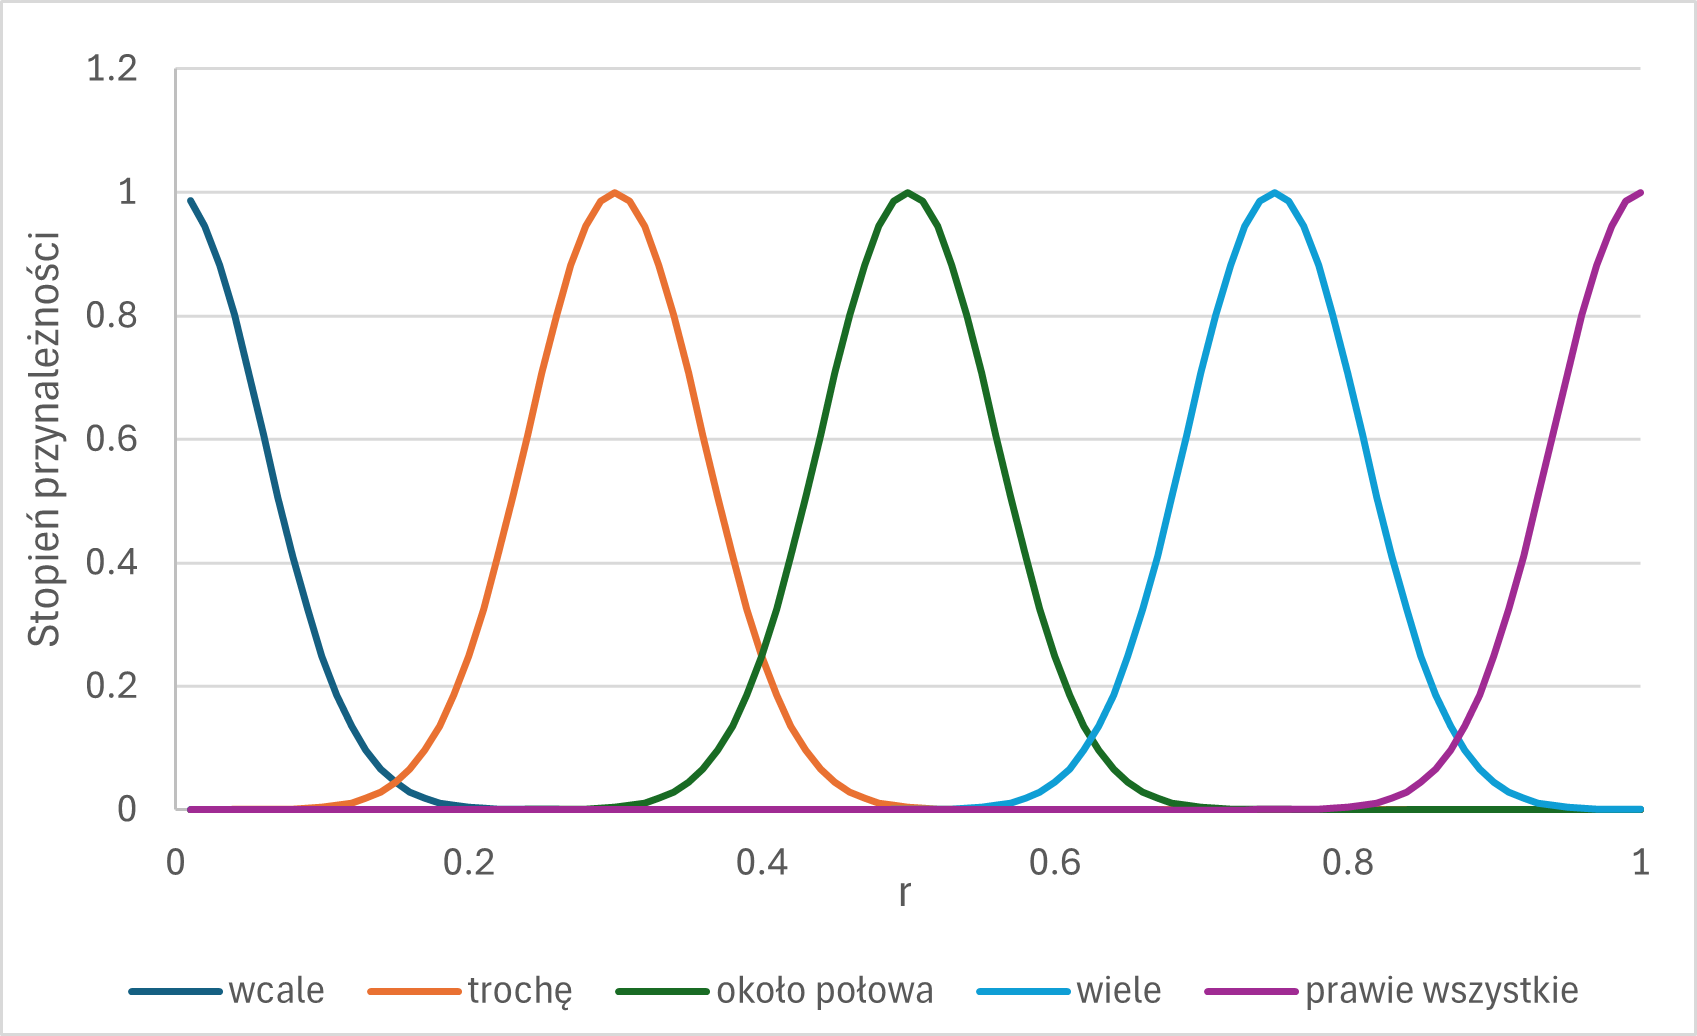
\includegraphics[width=0.7\textwidth]{img/a.png}
    \caption{Wykres funkcji przynależności dla kwantyfikatorów}
\end{figure}



\section{Narzędzia obliczeniowe: wybór/implementacja. Diagram UML klas do obliczeń rozmytych i generowania podsumowań}
Program został napisany w języku Java w wersji JDK 24. Do obsługi relacyjnej bazy danych PostgreSQL wykorzystano framework Spring Boot, który umożliwia wygodną konfigurację połączenia z bazą danych. Kod źródłowy komponentu odpowiedzialnego za obliczenia rozmyte został umieszczony w pakiecie o nazwie \texttt{fuzzy}. Znajduje sie w nim podstawowy model reprezentujący zbiory rozmyte, którego centralnym elementem jest abstrakcyjna klasa \texttt{FuzzySet}, która definiuje fundamentalne operacje na zbiorach rozmytych. Klasa ta udostępnia metody pozwalające na obliczanie podstawowych właściwości zbioru rozmytego, m.in. takich jak kardynalność oraz nośnik. Na bazie klasy \texttt{FuzzySet} zbudowane zostały trzy klasy reprezentujące konkretne typy funkcji przynależności: \texttt{GaussianFunction}, \texttt{TrapezoidalFunction} oraz \texttt{TriangularFunction}. Każda z tych klas implementuje matematyczną funkcję przynależności o charakterystycznym kształcie: odpowiednio gaussowskim, trapezoidalnym i trójkątnym. Dzięki temu możliwe jest precyzyjne modelowanie różnych pojęć językowych. \\
Oprócz modelu zbiorów rozmytych, pakiet \texttt{fuzzy} zawiera również klasy odpowiedzialne za tworzenie i przetwarzanie podsumowań lingwistycznych. Klasa \texttt{LinguisticVariable} reprezentuje zmienną lingwistyczną, która zawiera nazwę, przestrzeń rozważań oraz zestaw powiązanych z nią terminów lingwistycznych, np. „bardzo zimno”, „ciepło”, „gorąco”, które są reprezentowane przez odpowiednie zbiory rozmyte.
W strukturze podsumowań lingwistycznych wyróżniamy także kwalifikatory i sumaryzatory, które mają bardzo podobną strukturę, ponieważ są złożone z nazwy oraz przypisanego im zbioru rozmytego. Ich różnice wynikają jedynie z zastosowania, w jaki sposób są wykorzystywane w podsumowaniach lingwistycznych. W celu zachowania przejrzystości i uniknięcia duplikacji kodu, stworzona została wspólna klasa bazowa \texttt{LinguisticTerm}. 
Klasa \texttt{Quantifier} odpowiada za reprezentację kwantyfikatorów, takich jak „około połowy” czy „prawie żaden”. Kwantyfikator opisany jest za pomocą nazwy, funkcji przynależności oraz typu — może być kwantyfikatorem absolutnym lub względnym.
Kolejnym elementem pakietu jest klasa \texttt{SingleSubjectSummary}. To ona odpowiada za generowanie jednopodmiotowych podsumowań lingwistycznych oraz obliczanie miar jakości na podstawie przekazanych obiektów: sumaryzatora, kwalifikatora oraz kwantyfikatora. \\
Ostanim elementem jest klasa \texttt{DoubleSubjectSummary}, która generuje dwupodmiotowe podsumowania lingwistyczne wraz z ich miarami. \\
Strukturę logiczną opisanych klas oraz zależności między nimi przedstawiono diagramie UML dostępnym w załączniku lingustic.png.



\section{ Jednopodmiotowe podsumowania lingwistyczne. Miary jakości, podsumowanie optymalne}
Poniżej zaprezentowano wyniki eksperymentów polegających na generowaniu jednopodmiotowych podsumowań lingwistycznych. Eksperymenty zostały podzielone na trzy części. W każdym eksperymencie wykorzystano tylko kwalifikator relatywny. Dla każdego utworzonego podsumowania lingwistycznego obliczane były miary jakości oraz miara podsumowania optymalnego. W każdej z poniższych sekcji w tabelach przedstawiono wybrane podsumowania, dla których wartość miary \textit{degree of truth} (\(T_1\)) dla danego kwantyfikatora nie była mniejsza niż 0{,}01. \\
W tabelach zaprezentowano treść podsumowania oraz wartość optymalnej miary, która jest obliczana na podstawie sumy iloczynów wag i wartości pozostałych miar (\(T_1\)–\(T_{11}\)). Pozostałe miary jakości zostały załączone w pliku \textit{Załącznik3.pdf}. W celu obliczenia miary podsumowania optymalnego przyjęto następujące wagi: \(w1 = 0.30\), \(w2 = 0.07\), \(w3 = 0.07\), \(w4 = 0.07\), \(w5 = 0.07\), \(w6 = 0.07\), \(w7 = 0.07\), \(w8 = 0.07\), \(w9 = 0.07\), \(w_{10} = 0.07\), \(w_{11} = 0.70\).


\subsection{Podsumowania lingwistyczne pierwszego typu}
W tej sekcji zostały przedstawione wyniki dla podsumowań lingwistycznych z jednym sumaryzatorem.\\
W tabeli nr.2 przedstawiono miary jakości oraz miarę podsumowania optymalnego dla podsumowania lingwistycznego nr.1 z tabeli nr.1. Zdanie: \textit{„Prawie żaden pomiarów jest/ma zimną temperaturę”} zostało ocenione na podstawie następujących wskaźników: \(T_1\) – degree of truth, \(T_2\) – degree of imprecision (0{,}88), \(T_3\) – degree of covering, \(T_4\) – degree of appropriateness, \(T_5\) – length of summary (1{,}0), \(T_6\) – degree of quantifier imprecision, \(T_7\) – degree of quantifier cardinality, \(T_8\), \(T_9\) - degree of qualifier imprecision, \(T_{10}\) - degree of qualifier cardinality, \(T_{11}\), (\(T\)) - miara podsumowania optymalnego. Znaczenia wartości odpowiednich miar zostały opisane w sekcji 6.1.

\begin{table}[H]
    \centering
    \normalsize
    \begin{tabular}{|c|p{8cm}|c|c|}
    \hline
    \textbf{Lp.} &\textbf{Podsumowanie} & \textbf{\(T_1\)} & \textbf{T} \\ \hline
    1. & Prawie żaden pomiarów jest/ma zimną temperaturę & 0.54 & 0.59 \\ \hline
    2. & Około połowy pomiarów jest/ma ciepła temperaturę & 0.43 & 0.49 \\ \hline
    3. & Trochę pomiarów  jest/ma popołudniową godzinę & 0.92 & 0.66 \\ \hline
    4. & Prawie żaden pomiarów jest/ma wieczorną godzinę & 0.66 & 0.63 \\ \hline
    5. & Prawie żaden pomiarów jest/ma suche powietrze & 0.05 & 0.31 \\ \hline
    6. & Trochę pomiarów jest/ma suche powietrze & 0.30 & 0.37 \\ \hline
    7. & Prawie żaden pomiarów jest/ma silny wiatr & 0.66 & 0.63 \\ \hline
    8. & Około połowy pomiarów jest/ma słaby wiatr & 0.37 & 0.49 \\ \hline
    9. & Prawie wszystkie pomiarów jest/ma normalne cieśnienie & 0.70 & 0.56 \\ \hline
    10. & Prawie żaden pomiarów  jest/ma wysokie cisnienie & 0.73 & 0.66 \\ \hline
    11. & Prawie wszystkie pomiarów jest/ma umiarkowana widoczność & 0.68 & 0.55 \\ \hline
    12. & Prawie żaden pomiarów jest/ma dobra widoczność & 0.99 & 0.73 \\ \hline
    13. & Prawie wszystkie pomiarów  jest/ma normalne zanieczyszczenie NO2 & 0.72 & 0.46 \\ \hline
    14. & Około połowy pomiarów  jest/ma normalne zanieczyszczenie CO2 & 0.74 & 0.60 \\ \hline
    15. & Prawie żaden pomiarów  jest/ma niezdrowe zanieczyszczenie NO2 & 0.76 & 0.66 \\ \hline

    \end{tabular}
    \caption{Wyniki jednopodmiotowych podsumowań lingwistycznych typu 1 z \textit{degree of truth}.}
\end{table}

  \begin{table}[H]
    \centering
    \begin{tabular}{|c|c|c|c|c|c|c|c|c|c|c|c|}
    \hline
    \textbf{\(T_1\)} &\textbf{\(T_2\)} & \textbf{\(T_3\)} & \textbf{\(T_4\)} & \textbf{\(T_5\)} & \textbf{\(T_6\)} & \textbf{\(T_7\)} & \textbf{\(T_8\)} & \textbf{\(T_9\)} & \textbf{\(T_{10}\)} & \textbf{\(T_{11}\)} & \textbf{\(T\)} \\ \hline
    0.54 & 0.88 & 0.12 & 0.00 & 1.00 & 0.80 & 0.60 & 0.93 & 0.00 & 0.00 & 0.00 & 0.59 \\ \hline
    \end{tabular}
    \caption{Miary jakości dla podsumowania nr. 1 z tabeli nr.1.}
\end{table}  

\subsection{Podsumowania lingwistyczne pierwszego typu z dwoma sumaryzatorami}
W tej sekcji zostały przedstawione wyniki dla podsumowań lingwistycznych z dwoma sumaryzatorami.\\
W tabeli nr.4 przedstawiono miary jakości oraz miarę podsumowania optymalnego dla podsumowania lingwistycznego nr.4 z tabeli nr.3. Zdanie: \textit{„Około połowy pomiarów  jest/ma umiarkowany waitr i jest/ma normalne ciśnienie powietrza”}. Wszystkie miary zostały opisane w sekcji 6.1.


\begin{table}[H]
\begin{center}
\normalsize % lub \Large, \normalsize, itp.
\begin{tabular}{|c|p{8cm}|c|c|} % p{10cm} = zawijanie tekstu, szerokość dostosuj
\hline
\textbf{Lp.} & \textbf{Podsumowanie} & \textbf{\(T_1\)} & \textbf{T} \\ \hline
1. & Trochę pomiarów jest/ma ciepła temperaturę i jest/ma popołudniowa godzinę & 0.43 & 0.34 \\ \hline
2. & Prawie żaden pomiarów jest/ma ciepła temperaturę i jest/ma umiarkowane UV & 0.32 & 0.33 \\ \hline
3. & Prawie żaden pomiarów jest/ma wieczorną godzinę i jest/ma dobrą widoczność & 0.99 & 0.55 \\ \hline
4. & Około połowy pomiarów  jest/ma umiarkowany waitr i jest/ma normalne ciśnienie powietrza & 0.94 & 0.49 \\ \hline
5. & Trochę pomiarów jest/ma popołudniowa godzinę i jest/ma normalne ciśnienie powietrza & 0.90 & 0.47 \\ \hline
6. & Około połowy pomiarów jest/ma ciepła temperaturę i jest/ma normalne ciśnienie  powietrza & 0.45 & 0.33 \\ \hline
7. & Wiele pomiarów  jest/ma normalne zanieczyszczenie CO2 i jest/ma normalne ciśnienie powietrza & 0.28 & 0.27 \\ \hline
8. & wiele pomiarów  jest/ma umiarkowana jakość powietrza i jest/ma normalne zanieczyszczenie NO2 & 0.31 & 0.28 \\ \hline
9. & Prawie wszystkie pomiarów  jest/ma umiarkowana widoczność i jest/ma normalne zanieczysczenie NO2 & 0.26 & 0.28 \\ \hline
10. & Prawie wszystkie pomiarów  jest/ma normalne zanieczysczenie NO2 i jest/ma normalne ciśnienie powietrza & 0.31 & 0.30 \\ \hline
\end{tabular}
\caption{Wyniki jednopodmiotowych podsumowań lingwistycznych typu 1 z dwoma sumaryzatorami z miarą \textit{degree of truth}.}
\end{center}
\end{table}

\begin{table}[H]
    \centering
    \begin{tabular}{|c|c|c|c|c|c|c|c|c|c|c|c|}
    \hline
    \textbf{\(T_1\)} &\textbf{\(T_2\)} & \textbf{\(T_3\)} & \textbf{\(T_4\)} & \textbf{\(T_5\)} & \textbf{\(T_6\)} & \textbf{\(T_7\)} & \textbf{\(T_8\)} & \textbf{\(T_9\)} & \textbf{\(T_{10}\)} & \textbf{\(T_{11}\)} & \textbf{\(T\)} \\ \hline
    0.94 & 0.01 & 0.99 & 0.00 & 0.50 & 0.60 & 0.62 & 0.29 & 0.00 & 0.00 & 0.00 & 0.49 \\ \hline
    \end{tabular}
    \caption{Miary jakości dla podsumowania nr. 4 z tabeli nr.3.}
\end{table}  


\subsection{Podsumowania lingwistyczne drugiego typu z jednym sumaryzatorem}
W tej sekcji zostały przedstawione wyniki dla podsumowań lingwistycznych z jednym sumaryzatorem i jednym kwalifikatorem.\\
W tabeli nr.6 przedstawiono miary jakości oraz miarę podsumowania optymalnego dla podsumowania lingwistycznego nr.9 z tabeli nr.5. Zdanie: \textit{„Prawie wszystkie pomiarów będący/mający gorąca temperaturę jest/ma normalne zanieczysczenie NO2”}, wszystkie przedstawione w niej miary zostały opisane w sekcji 6.1. 


\begin{table}[H]
\begin{center}
\normalsize % lub \Large, \normalsize, itp.
\begin{tabular}{|c|p{8cm}|c|c|} % p{10cm} = zawijanie tekstu, szerokość dostosuj
\hline
\textbf{Lp.} & \textbf{Podsumowanie} & \textbf{\(T_1\)} & \textbf{T} \\ \hline
1. & Prawie żaden pomiarów będący/mający wieczorna godzinę jest/ma bardzo silny wiatr & 1.0 & 0.81\\\hline
2. & Prawie żaden pomiarów będący/mający ciepła temperature jest/ma umiarkowana widoczność & 0.69 & 0.63 \\ \hline
3. & Trochę pomiarów będący/mający ekstremalne UV jest/ma dobra jakość powietrza & 0.84 & 0.74 \\ \hline
4. & Trochę pomiarów będący/mający wysokie cisnienie jest/ma poranna godzine & 0.47 & 0.62 \\ \hline
5. & Około połowy pomiarów będący/mający południowa godzinę jest/ma słaby wiatr & 0.99 & 0.70 \\ \hline
6. & Około połowy pomiarów będący/mający normalne cisnienie jest/ma umiarkowany wiatr & 0.72 & 0.55 \\\hline
7. & Wiele pomiarów będący/mający ekstremalne UV jest/ma południowa godzinę & 0.20 & 0.57 \\ \hline
8. & Wiele pomiarów będący/mający niskie cisnienie jest/ma wilgotne powietrze & 0.42 & 0.56 \\ \hline
9. & Prawie wszystkie pomiarów będący/mający gorąca temperaturę jest/ma normalne zanieczysczenie NO2 & 0.86 & 0.70 \\ \hline
10. & Prawie wszystkie pomiarów będący/mający normalne zanieczysczenie NO2 jest/ma umiarkowana widoczność & 0.70 & 0.58 \\ \hline

\end{tabular}
\caption{Wyniki jednopodmiotowych podsumowań lingwistycznych typu 2 z miarą \textit{degree of truth}.}
\end{center}
\end{table}


\begin{table}[H]
    \centering
    \begin{tabular}{|c|c|c|c|c|c|c|c|c|c|c|c|}
    \hline
    \textbf{\(T_1\)} &\textbf{\(T_2\)} & \textbf{\(T_3\)} & \textbf{\(T_4\)} & \textbf{\(T_5\)} & \textbf{\(T_6\)} & \textbf{\(T_7\)} & \textbf{\(T_8\)} & \textbf{\(T_9\)} & \textbf{\(T_{10}\)} & \textbf{\(T_{11}\)} & \textbf{\(T\)} \\ \hline
    0.86 & 0.02 & 0.98 & 0.00 & 1.00 & 0.80 & 0.65 & 0.05 & 0.82 & 0.94 & 1.00 & 0.70 \\ \hline
    \end{tabular}
    \caption{Miary jakości dla podsumowania nr. 15 z tabeli nr.5.}
\end{table}  


\section{Wielopodmiotowe podsumowania lingwistyczne i~ich miary jakości} 
Poniżej zaprezentowano wyniki eksperymentów polegających na generowaniu wielopodmiotowych podsumowań lingwistycznych. Z bazy danych opisanej w sekcji 2.1 zostały wyodrębnione cztery podmioty, które dzielą podmiot główny - pomiar, na pomiar wykonany na danym kontynencie. Wyróżnione zostały cztery kontynenty - Europe, Asia, Africa, America. Podsumownania wielopodmiotowe będą generowane w czterech formach, ograniczając się przy tym do wykorzystania w tym samym momencie tylko dwóch podmiotów. W tabelach zaprezentowano treść podsumowania oraz wartość miary degree of truth, która za każdym razem opisuje prawdziwość danego wyrażenia.

\subsection{Dwupodmiotowe podsumowania w pierwszej formie}
W tej sekcji zostały przedstawione wyniki dla dwupodmiotowych podsumowań lingwistycznych z jednym sumaryzatorem.

\begin{table}[H]
\begin{center}
\normalsize % lub \Large, \normalsize, itp.
\begin{tabular}{|c|p{10cm}|c|} % p{10cm} = zawijanie tekstu, szerokość dostosuj
\hline
\textbf{Lp.} & \textbf{Podsumowanie} & \textbf{\(T_1\)} \\ \hline
1. & Prawie żaden pomiarów z Africa w porównaniu do pomiarów z America jest/ma bardzo zimna temperature & 1.0 \\\hline
2. & Prawie żaden pomiarów z Asia w porównaniu do pomiarów z Africa jest/ma poranna godzinę & 0.96 \\\hline
3. & Prawie żaden pomiarów z America w porównaniu do pomiarów z Asia jest/ma suche powietrze & 0.85 \\\hline
4. & Prawie żaden pomiarów z Asia w porównaniu do pomiarów z America jest/ma dobra widoczność & 0.62 \\\hline
5. & Trochę pomiarów z Asia w porównaniu do pomiarów z Europe jest/ma umiarkowana temperaturę & 0.95 \\\hline
6. & Trochę pomiarów z Europe w porównaniu do pomiarów z America jest/ma bardzo zimna temperaturę & 0.95 \\\hline
7. & Trochę pomiarów z America w porównaniu do pomiarów z Europe jest/ma gwałtowny  wiatr & 0.97 \\\hline
8. & Około połowy pomiarów z America w porównaniu do pomiarów z Europe jest/ma wysokie UV & 0.75 \\\hline
9. & Około połowy pomiarów z Europe w porównaniu do pomiarów z America jest/ma wysokie UV & 0.75 \\\hline
10. & Wiele pomiarów z Europe w porównaniu do pomiarów z Africa jest/ma umiarkowana temperaturę & 0.85 \\\hline
11. & Wiele pomiarów z Europe w porównaniu do pomiarów z Africa jest/ma słaba widoczność & 0.24 \\\hline
12. & Prawie wszystkie pomiarów z Europe w porównaniu do pomiarów z Africa jest/ma zimna temperaturę & 0.99 \\\hline
\end{tabular}
\caption{Wyniki dwupodmiotowych podsumowań lingwistycznych w pierwszej formie z miarą \textit{degree of truth}.}
\end{center}
\end{table}

\subsection{Dwupodmiotowe podsumowania w drugiej formie}
W tej sekcji zostały przedstawione wyniki dla dwupodmiotowych podsumowań lingwistycznych w drugiej formie.

\begin{table}[H]
\begin{center}
\normalsize % lub \Large, \normalsize, itp.
\begin{tabular}{|c|p{10cm}|c|} % p{10cm} = zawijanie tekstu, szerokość dostosuj
\hline
\textbf{Lp.} & \textbf{Podsumowanie} & \textbf{\(T_1\)} \\ \hline
1. & Prawie żaden pomiarów z Asia w porównaniu do pomiarów z Africa, które są/mają niezdrowe zanieczyszczenie CO2 jest/ma poranna godzinę & 0.96 \\\hline  
2. & Trochę pomiarów z Asia w porównaniu do pomiarów z Europe, które są/mają niezdrowe zanieczyszczenie CO2 jest/ma południowa godzinę & 0.83 \\\hline 
3. & Około połowy pomiarów z Africa w porównaniu do pomiarów z Europe, które są/mają wysokie ciśnienie jest/ma poranna godzinę & 0.43 \\\hline
4. & Około połowy pomiarów z Africa w porównaniu do pomiarów z Europe, które są/mają wysokie ciśnienie jest/ma popołudniowa godzinę & 0.34 \\\hline
5. & Wiele pomiarów z Asia w porównaniu do pomiarów z America, które są/mają niezdrowe zanieczysczenie NO2 jest/ma niezdrowe zanieczyszczenie CO2 & 0.82 \\\hline
6. & Wiele pomiarów z Asia w porównaniu do pomiarów z America, które są/mają umiarkowany wiatr jest/ma zimna temperaturę & 0.66 \\\hline 
\end{tabular}
\caption{Wyniki dwupodmiotowych podsumowań lingwistycznych w drugiej formie z miarą \textit{degree of truth}.}
\end{center}
\end{table}

\subsection{Dwupodmiotowe podsumowania w trzeciej formie}
W tej sekcji zostały przedstawione wyniki dla dwupodmiotowych podsumowań lingwistycznych w trzeciej formie.

\begin{table}[H]
\begin{center}
\normalsize % lub \Large, \normalsize, itp.
\begin{tabular}{|c|p{10cm}|c|} % p{10cm} = zawijanie tekstu, szerokość dostosuj
\hline
\textbf{Lp.} & \textbf{Podsumowanie} & \textbf{\(T_1\)} \\ \hline
1. & Prawie żaden pomiarów z Africa, które są/mają niezdrowe zanieczyszczenie NO2, w porównaniu do pomiarów z America jest/ma niebezpieczne zanieczyszczenie CO2 & 0.61 \\\hline
2. & Trochę pomiarów z Africa, które są/mają słaby wiatr, w porównaniu do pomiarów z Europe jest/ma niskie UV & 1.0 \\\hline
3. & Trochę pomiarów z America, które są/mają słaby wiatr, w porównaniu do pomiarów z Europe jest/ma niskie UV & 0.76 \\\hline
4. & Około połowy pomiarów z Asia, które są/mają wilgotne powietrze, w porównaniu do pomiarów z Africa jest/ma wysokie UV & 0.96 \\\hline
5. & Wiele pomiarów z Asia, które są/mają wilgotne powietrze, w porównaniu do pomiarów z Europe jest/ma niskie UV & 0.51 \\\hline
6. & Prawie wszystkie pomiarów z Asia, które są/mają wilgotne powietrze, w porównaniu do pomiarów z Europe jest/ma bardzo dobra jakość powietrza & 0.91 \\\hline
\end{tabular}
\caption{Wyniki dwupodmiotowych podsumowań lingwistycznych w trzeciej formie z miarą \textit{degree of truth}.}
\end{center}
\end{table}

\subsection{Dwupodmiotowe podsumowania w czwartej formie}
W tej sekcji zostały przedstawione wyniki dla dwupodmiotowych podsumowań lingwistycznych w czwartej formie.

\begin{table}[H]
\begin{center}
\normalsize % lub \Large, \normalsize, itp.
\begin{tabular}{|c|p{10cm}|c|} % p{10cm} = zawijanie tekstu, szerokość dostosuj
\hline
\textbf{Lp.} & \textbf{Podsumowanie} & \textbf{\(T_1\)} \\ \hline
1. & Więcej pomiarów z Asia niż pomiarów z Africa jest/ma ciepła temperaturę & 0.67 \\\hline
2. & Więcej pomiarów z Asia niż pomiarów z Africa jest/ma bardzo silny wiatr & 0.49 \\\hline
3. & Więcej pomiarów z America niż pomiarów z Europe jest/ma bardzo zła jakość powietrza & 0.59 \\\hline
4. & Więcej pomiarów z Europe niż pomiarów z Africa jest/ma normalne ciśnienie & 0.55 \\\hline
5. & Więcej pomiarów z America niż pomiarów z Europe jest/ma niskie UV & 0.75 \\\hline
6. & Więcej pomiarów z America niż pomiarów z Europe jest/ma niezdrowe zanieczyszczenie CO2 & 0.58 \\\hline 
\end{tabular}
\caption{Wyniki dwupodmiotowych podsumowań lingwistycznych w czwartej formie z miarą \textit{degree of truth}.}
\end{center}
\end{table}

\section{Dyskusja, wnioski}

\subsection{Jednopodmiotowe podsumowania lingwistyczne}
Etap generowania jednopodmiotowych podsumowań lingwistycznych był podzielony na trzy etapy. W pierwszym z nich były generowane podsumowania pierwszego typu z jednym sumaryzatorem. W tym doświadczeniu wygenerowano podsumowania dla każdego możliwego zbioru rozmytego danej zmiennej lingwistycznej z wszystkimi kwantyfikatorami. Natomiast uwaga była poświęcona tylko tym podsumowaniom, które uzyskały \(T_1\) > 0.01. Na początku warto zauważyć, że znacznie więcej pojawiało się podsumowań z kwantyfikatorem \textit{"prawie żaden"} lub \textit{"trochę"} w porównaniu do kwantyfikatów opisanych poprzez \textit{"wiele"}, \textit{"prawie wszystkie"}. Taka sytuacja pozwala dostrzec jakie cechy pojawiają się w bazie rzadko, np. \textit{"zimna temperatura"}, \textit{"niezdrowe zanieczyszczenie NO2"}, z czego ta druga cecha prowadzi do ciekawych wniosków, że powietrze w badanych regionach jest rzadko zanieczyszczone tlenkiem NO2. Pozwala to także zauważyć jakie cechy pojawiają się często, np. \textit{"normalne ciśnienie"}, \textit{"normalne zanieczyszczenie NO2"}. W przeprowadzonych doświadczeniach warto zwrócić uwagę na dwa podsumowania, \textit{"Prawie żaden pomiarów jest/ma suche powietrze"} oraz \textit{"Trochę pomiarów jest/ma suche powietrze"} i na ich miary \(T_1\), odpowiednio (0,05) i (0.30), przy poprawnym skonstruowaniu modelu funkcji kwantyfikatorów te wartości po zsumowaniu powinny wynosić (1.00). Każde podsumowanie posiada 12 miar oceniających jakość, przy czym miara \(T_1\) została uznana za najistotniejszą, jako ta, która ma największe znaczenie dla wiarygodności otrzymanego podsumowania. I tak w zdaniu \textit{"Prawie żaden pomiarów jest/ma zimną temperaturę"} \(T_1\) = (0.54), co oznacza, że podsumowanie jest zgodne z danymi w 54\%. Zgodnie z tabelą nr. 2 wspomniane wcześniej podsumowanie dla miary \(T_2\) = (0.88), czyli sumaryzator \textit{"zimna temperatura"} jest bardzo nieprecyzyjny. \(T_3\) = (0.12), czyli niewielka część danych spełnia warunki zawarte w podsumowaniu, co jest zgodne z przyjętym kwantyfikatorem \textit{"prawie żaden"}. \(T_4\) = (0.00), taka wartość z powodu tylko jednego sumaryzatora. \(T_5\) = 1.0, czyli w podsumowaniu występuje dokładnie jeden sumaryzator. \(T_6\) = 0.8, wykorzystany kwantyfikator \textit{"prawie żaden"} jest precyzyjny. \(T_7\) = 0.6, oznacza umiarkowaną liczebność obiektów w kwantyfikatorze wykorzystanym w tym podsumowaniu. \(T_8\) = (0.94) oznacza, że sumaryzator słabo odpowiada danym zawartym w bazie danych. Miary \(T_9\), \(T_{10}\) i \(T_{11}\) są równe (0.00), ponieważ podsumowanie nie zawiera kwalifikatora. Ostateczna miara jakości podsumowania (\(T\)) wynosi (0{.}61), co sugeruje umiarkowanie dobrą jakość wygenerowanego podsumownania. \\
W drugim doświadczeniu tworzono podsumowania z wykorzystaniem dwóch sumaryzatorów. Podobnie jak w przypadku pierwszego doświadczenia, jednak w tym przypadku dużo większa część podsumowań lingwistycznych była oznaczona przez kwantyfikator \textit{"prawie żaden"} lub \textit{"trochę"}. Jest to związane z tym, że dużo ciężej stworzyć takie podsumowanie, które odpowiada jednocześnie dwóm cechom. Na wszystkie możliwe kombinacje podsumowań lingwistycznych z dwoma sumaryzatorami tylko 6 posiadało kwantyfikator \textit{"prawie wszystkie"} lub \textit{"wiele"}. Warte wspomnienia jest tutaj m.in. zdanie \textit{"Prawie wszystkie pomiarów jest/ma normalne zanieczyszczenie CO2 i normalne ciśnienie powietrza"}, które niesie bardzo konkretną informację o dobrych warunkach atmosferycznych. Warte uwagi jest zdanie \textit{"Prawie żaden pomiarów jest/ma wieczorną godzinę i jest/ma dobrą widoczność"}, które jest bardzo logicznym zdaniem, ponieważ zwykle w wieczornych godzinach, kiedy jest ciemno, to widoczność jest ograniczona. Miary jakości dla zdania \textit{„Około połowy pomiarów jest/ma normalne ciśnienie i jest/ma umiarkowany wiatr”} przedstawione w tabeli nr. 4 niosą ze sobą następujące informacje. \(T_1\) = (0.94) czyli to podsumowanie jest bardzo zgodne z tym, co reprezentują dane w bazie danych. Następnie \(T_2\) = (0.01) sugeruje że obydwa sumaryzatory \textit{"normalne ciśnienie powietrza"} oraz \textit{"umiarkowany wiatr"} są bardzo precyzyjnie określone. \(T_3\) = (0.99) miara która oznacza, że znaczna część danych spełnia warunki podsumowania. \(T_4\) =  (0.00). \(T_5\) = (0.5) - dwa sumaryzatory w jednym podsumowaniu. \(T_6\) = (0.6), wykorzystywany kwantyfikator \textit{"około połowy"} jest mniej precyzyjny w porównaniu do kwantyfikatora opisanego w poprzednim doświadczeniu (\textit{"prawie żaden"} miał \(T_6\) = (0.80)). \(T_7\) = (0.62) oznacza umiarkowaną liczebność obiektów w kwantyfikatorze wykorzystanym w tym podsumowaniu. \(T_8\) = (0.29), wykorzystane sumaryzatory dobrze odpowiadają danym zawartym w bazie danych. Miary \(T_9\), \(T_{10}\) i \(T_{11}\) są równe (0.00), ponieważ podsumowanie nie zawiera kwalifikatora. Ostateczna miara jakości podsumowania (\(T\)) wynosi (0{.}49), i jest nieco gorsza niż ta w przypadku przykładu podsumownia lingwistycznego z jednym sumaryzatorem. \\
W kolejnym doświadczeniu badano jednopodmiotowe podsumowania lingwistyczne drugiego typu, czyli takie, które składają się z kwalifikatora i sumaryzatora. Podobnie jak w poprzednim doświadczeniu wygenerowano podsumowania lingwistyczne dla każdej możliwej kombinacji kwalifikatora z sumaryzatorem. Natomiast liczebności uzyskanych podsumowań dla kolejnych kwantyfikatorów nie różnią się tak drastycznie od siebie. Dla przykładu dla kwantyfikatora \textit{"wiele"} udało się uzyskać aż 116 podsumowań. Jest to oczywiście związane z tym, że podsumownia w drugiego typu nie skupiają się na informacjach ogólnych, tylko na tych obiektach z bazy danych, które spełniają dany kwalifikator. W zdaniu \textit{"Wiele pomiarów będący/mający ekstremalne UV jest/ma południowa godzinę"} rozpatrywane są tylko te obiekty, które w pierwszej kolejności spełniają wymóg kwalifikatora, czyli \textit{"eksremalne UV"}. Miary jakości dla zdania \textit{„Prawie wszystkie pomiarów będący/mający gorąca temperaturę jest/ma normalne zanieczysczenie NO2”} przestawione w tabeli nr.6 mają następujące znaczenie. \(T_1\) = (0.86), czyli 86\% danych spełnia założenia kwalifikatora \textit{"gorąca temperatura"} i sumaryzatora \textit{"normalne zanieczysczenie NO2"}. \(T_2\) = (0.02), czyli sumaryzator jest precyzyjnie określony, \(T_3\) = (0.99), czyli prawie wszystkie wiersze z bazy danych odpowiadających w pewnym stopniu kwalifikatorowi \textit{"gorąca temperatura"} jest objętych tym podsumowaniem.\(T_4\) = (0.00), taka wartość z powodu tylko jednego sumaryzatora. \(T_5\) = (1.00), jeden sumaryzator. \(T_6\) = (0.80), co oznacza, że kwantyfikator \textit{"prawie wszystkie"} jest precyzyjny. \(T_7\) = (0.65) oznacza umiarkowaną liczebność obiektów w kwantyfikatorze wykorzystanym w tym podsumowaniu. \(T_8\) = (0.05), wykorzystany sumaryzator bardzo dobrze odpowiada danym zawartym w bazie danych. \(T_9\) = (0.82) oznacza, że kwalifikator jest nieprecyzjny, im wyższa wartość tym gorzej. \(T_{10}\) = (0.94), co oznacza, że wiele obiektów jest objęte kwalifikatorem \textit{"gorąca temperatura"}. \(T_{11}\) = (1.00), czyli w podsumowaniu został wykorzystany jeden kwalifikator. \(T\) = (0.70), czyli wartość miary optymalnej jest dobra w porównaniu z tym, co zostało opisane w przypadku podsumowań pierwszego typu z jednym i dwoma sumaryzatorami. 

\subsection{Wielopodmiotowe podsumowania lingwistyczne}
Wielopodmiotowe podsumowania lingwistyczne były generowane w czterech różnych formach. Pierwsza z nich dotyczyła podsumowania, w którym występują dwa podmioty i jeden sumaryzator. Przeprowadzone doświadczenie doprowadziło do ciekawych rezultatów, mianowicie w przeciwieństwie do jednopodmiotowych podsumowań lingwistycznych, liczba podsumowań wygenerowanych z miarą \(T_1\)> 0.01 dla kwantyfikatórów \textit{"prawie żaden"} oraz \textit{"trochę} nie jest dominująca. W tym przypadku uzyskano najwięcej podsumowań dla kwantyfikatora \textit{"około połowy"}. Podział bazy danych na cztery podzbiory pozwolił na uzyskanie dużo bardziej szczegółowych informacji dotyczących pomiarów. Np. podsumowanie \textit{"Prawie wszystkie pomiarów z Europe w porównaniu do pomiarów z Africa jest/ma zimna temperaturę"} \(T_1 = 0.99\) potwierdza bardzo intuicyjne skojarzenie na temat temperatur, jakie występują  w Europie i Afryce. Natomiast podsumowanie \textit{"Prawie żaden pomiarów z America w porównaniu do pomiarów z Asia jest/ma suche powietrze"} nie jest od razu oczywiste, że klimat amerykański jest suchszy od azjatyckiego. \\
Podsumowania wielopodmiotowe w drugiej oraz trzeciej formie pozwalają na jeszcze większe uszczegółowienie informacji, jakie niosą ze sobą te podsumowania. Występuje tutaj kwalifikator, który dotyczy pierwszego albo drugiego podmiotu. Dzięki temu możliwe jest nie tylko porównanie dwóch różnych grup, ale również uwzględnienie określonej cechy charakteryzującej jedną z nich, co znacząco zwiększa wartość informacyjną takich podsumowań. W drugiej formie kwalifikator odnosi się do drugiego podmiotu. Przykładowo, podsumowanie: \textit{"Trochę pomiarów z Asia w porównaniu do pomiarów z Europe, które są/mają niezdrowe zanieczyszczenie CO2, jest/ma południową godzinę”} \(T_1 = 0.83\)
wskazuje, że tylko niewielka część pomiarów z Azji, w porównaniu do tych z Europy spełniających określony warunek, ma daną cechę. Wartość stopnia prawdziwości na poziomie 0.83 świadczy o dość wysokiej zgodności tej informacji z danymi źródłowymi. Z kolei w trzeciej formie kwalifikator odnosi się do pierwszego podmiotu. Taka struktura pozwala określić, jaka część pierwszego podmiotu (z uwzględnieniem jego właściwości) różni się od drugiego. Przykład: \textit{"Prawie wszystkie pomiarów z Asia, które są/mają wilgotne powietrze, w porównaniu do pomiarów z Europe, jest/ma bardzo dobrą jakość powietrza”}. Miara \(T_1 = 0.91\) pokazuje, że większość pomiarów z Azji, w warunkach wilgotnego powietrza, ma lepszą jakość powietrza niż Europa i to z dużą zgodnością z obiektami z bazy danych. \\
Ostatnia - czwarta forma określa czy dany podmiot na więcej elementów spełniających warunki danego sumaryzatora. W przypadku tego typu podsumowań należy zwrócić uwagę na liczebności danych podzbiorów, ponieważ duża dysproporcja może doprowadzić do tego, ze dany podmiot nie będzie miał więcej obiektów dla żadnego sumaryzatora. Na podstawie przeprowadzonych doświadczeń otrzymano dla przykładu: \textit{"Więcej pomiarów z Asia niż pomiarów z Africa jest/ma ciepła temperaturę"} z miarą \(T_1 = 0.67\), która oznacza, że rzeczywiście pomiary dokonane w Azji przeważają liczebnością w aspekcie ciepłej temperatury w stosunku do Afryki. Natomiast w przypadku tego podsumowania: \textit{"Więcej pomiarów z Asia niż pomiarów z Africa jest/ma bardzo silny wiatr"} miara \(T_1 = 0.49\) oznacza, że Azja niekoniecznie ma przewagę w liczebności pomiarów posiadających silny wiatr.

\subsection{Wnioski}
\begin{itemize}
    \item Miara \(T_1\) przekazuje najistotniejsze informacje na temat dokonanych podsumowań. 
    \item Podczas generowania jednopodmiotowych podsumowań lingwistycznych dużo częściej pojawią sie te z kwantyfikatorem \textit{"prawie żaden"} lub \textit{"trochę"}.
    \item Znacznie trudniej wygenerować wysokiej jakości podsumowania spełniające dwie lub więcej cech.
    \item Wartości stopnia przynależności dla kolejnych kwantyfikatorów powinny przecinać się w połowie.
    \item Podsumowania jednopodmiotowe drugiego typu niosą za sobą dużo bardziej szczegółowe informacje.
    \item Generowanie wielopodmiotowych podsumowań lingwistycznych pozwala na uzyskanie dużo bardziej szczegółowych informacji.
    \item Podsumowania wielopodmiotowe, w przeciwieństwie do jednopodmiotowych, dają możliwość znalezienia zależności, pomiędzy niektórymi podmiotami w badanym zbiorze danych. 
\end{itemize}


\section{Braki w realizacji projektu 2.}
Wymienić wg opisu Projektu 2. wszystkie niezrealizowane obowiązkowe elementy projektu, ewentualnie
podać merytoryczne (ale nie czasowe) przyczyny tych braków. 


\begin{thebibliography}{99}
\bibitem{baza} World Weather Repository - kaggle, \url{https://www.kaggle.com/datasets/nelgiriyewithana/global-weather-repository?resource=download}. [dostęp 18.05.2025r.]
 \bibitem{niewiadomski19} A. Niewiadomski, Zbiory rozmyte typu 2. Zastosowania w reprezentowaniu informacji.  Seria „Problemy współczesnej informatyki” pod redakcją L. Rutkowskiego. Akademicka Oficyna Wydawnicza EXIT, Warszawa, 2019.
\bibitem{zadrozny06} S. Zadrożny, Zapytania nieprecyzyjne i lingwistyczne podsumowania baz danych, EXIT, 2006, Warszawa
\bibitem{niewiadomski08} A. Niewiadomski, Methods for the Linguistic Summarization of Data: Applications of Fuzzy Sets and Their Extensions, Akademicka Oficyna Wydawnicza EXIT, Warszawa, 2008.
\end{thebibliography}

Literatura zawiera wyłącznie źródła recenzowane i/lub o potwierdzonej wiarygodności,
możliwe do weryfikacji i cytowane w sprawozdaniu. 
\end{document}
